% Slides for 2025-08-12
% To create a slide, use the following:
% \begin{frame}{TITLE}
%     BODY
% \end{frame}

% To create a slide with a bullet list, use the following:
% \begin{frame}{TITLE}
%     \begin{itemize}
%         \item ITEM 1
%         \item ITEM 2
%     \end{itemize}    
% \end{frame}

% To create a slide with numbered list, use the following:
% \begin{frame}{TITLE}
%     \begin{enumerate}
%         \item ITEM 1
%         \item ITEM 2
%     \end{enumerate}
% \end{frame}

% To create a slide with a graphic:
% 1. Add the graphic to this folder (named picture.png)
% 2. Use the following:
% \begin{frame}{TITLE}
%     \centering
%     \includegraphics[height=0.7\textheight,width=0.7\textwidth,keepaspectratio]{picture.png}
% \end{frame}

% To create a slide with two columns, use the following:
% \begin{frame}{TITLE}
%     \begin{columns}
%         \begin{column}{0.5\textwidth}
%             COLUMN 1 BODY
%         \end{column}
%         \begin{column}{0.5\textwidth}
%             COLUMN 2 BODY
%         \end{column}
%     \end{columns}
% \end{frame}

\begin{frame}{DWE on Rubik Pi}
    \centering
    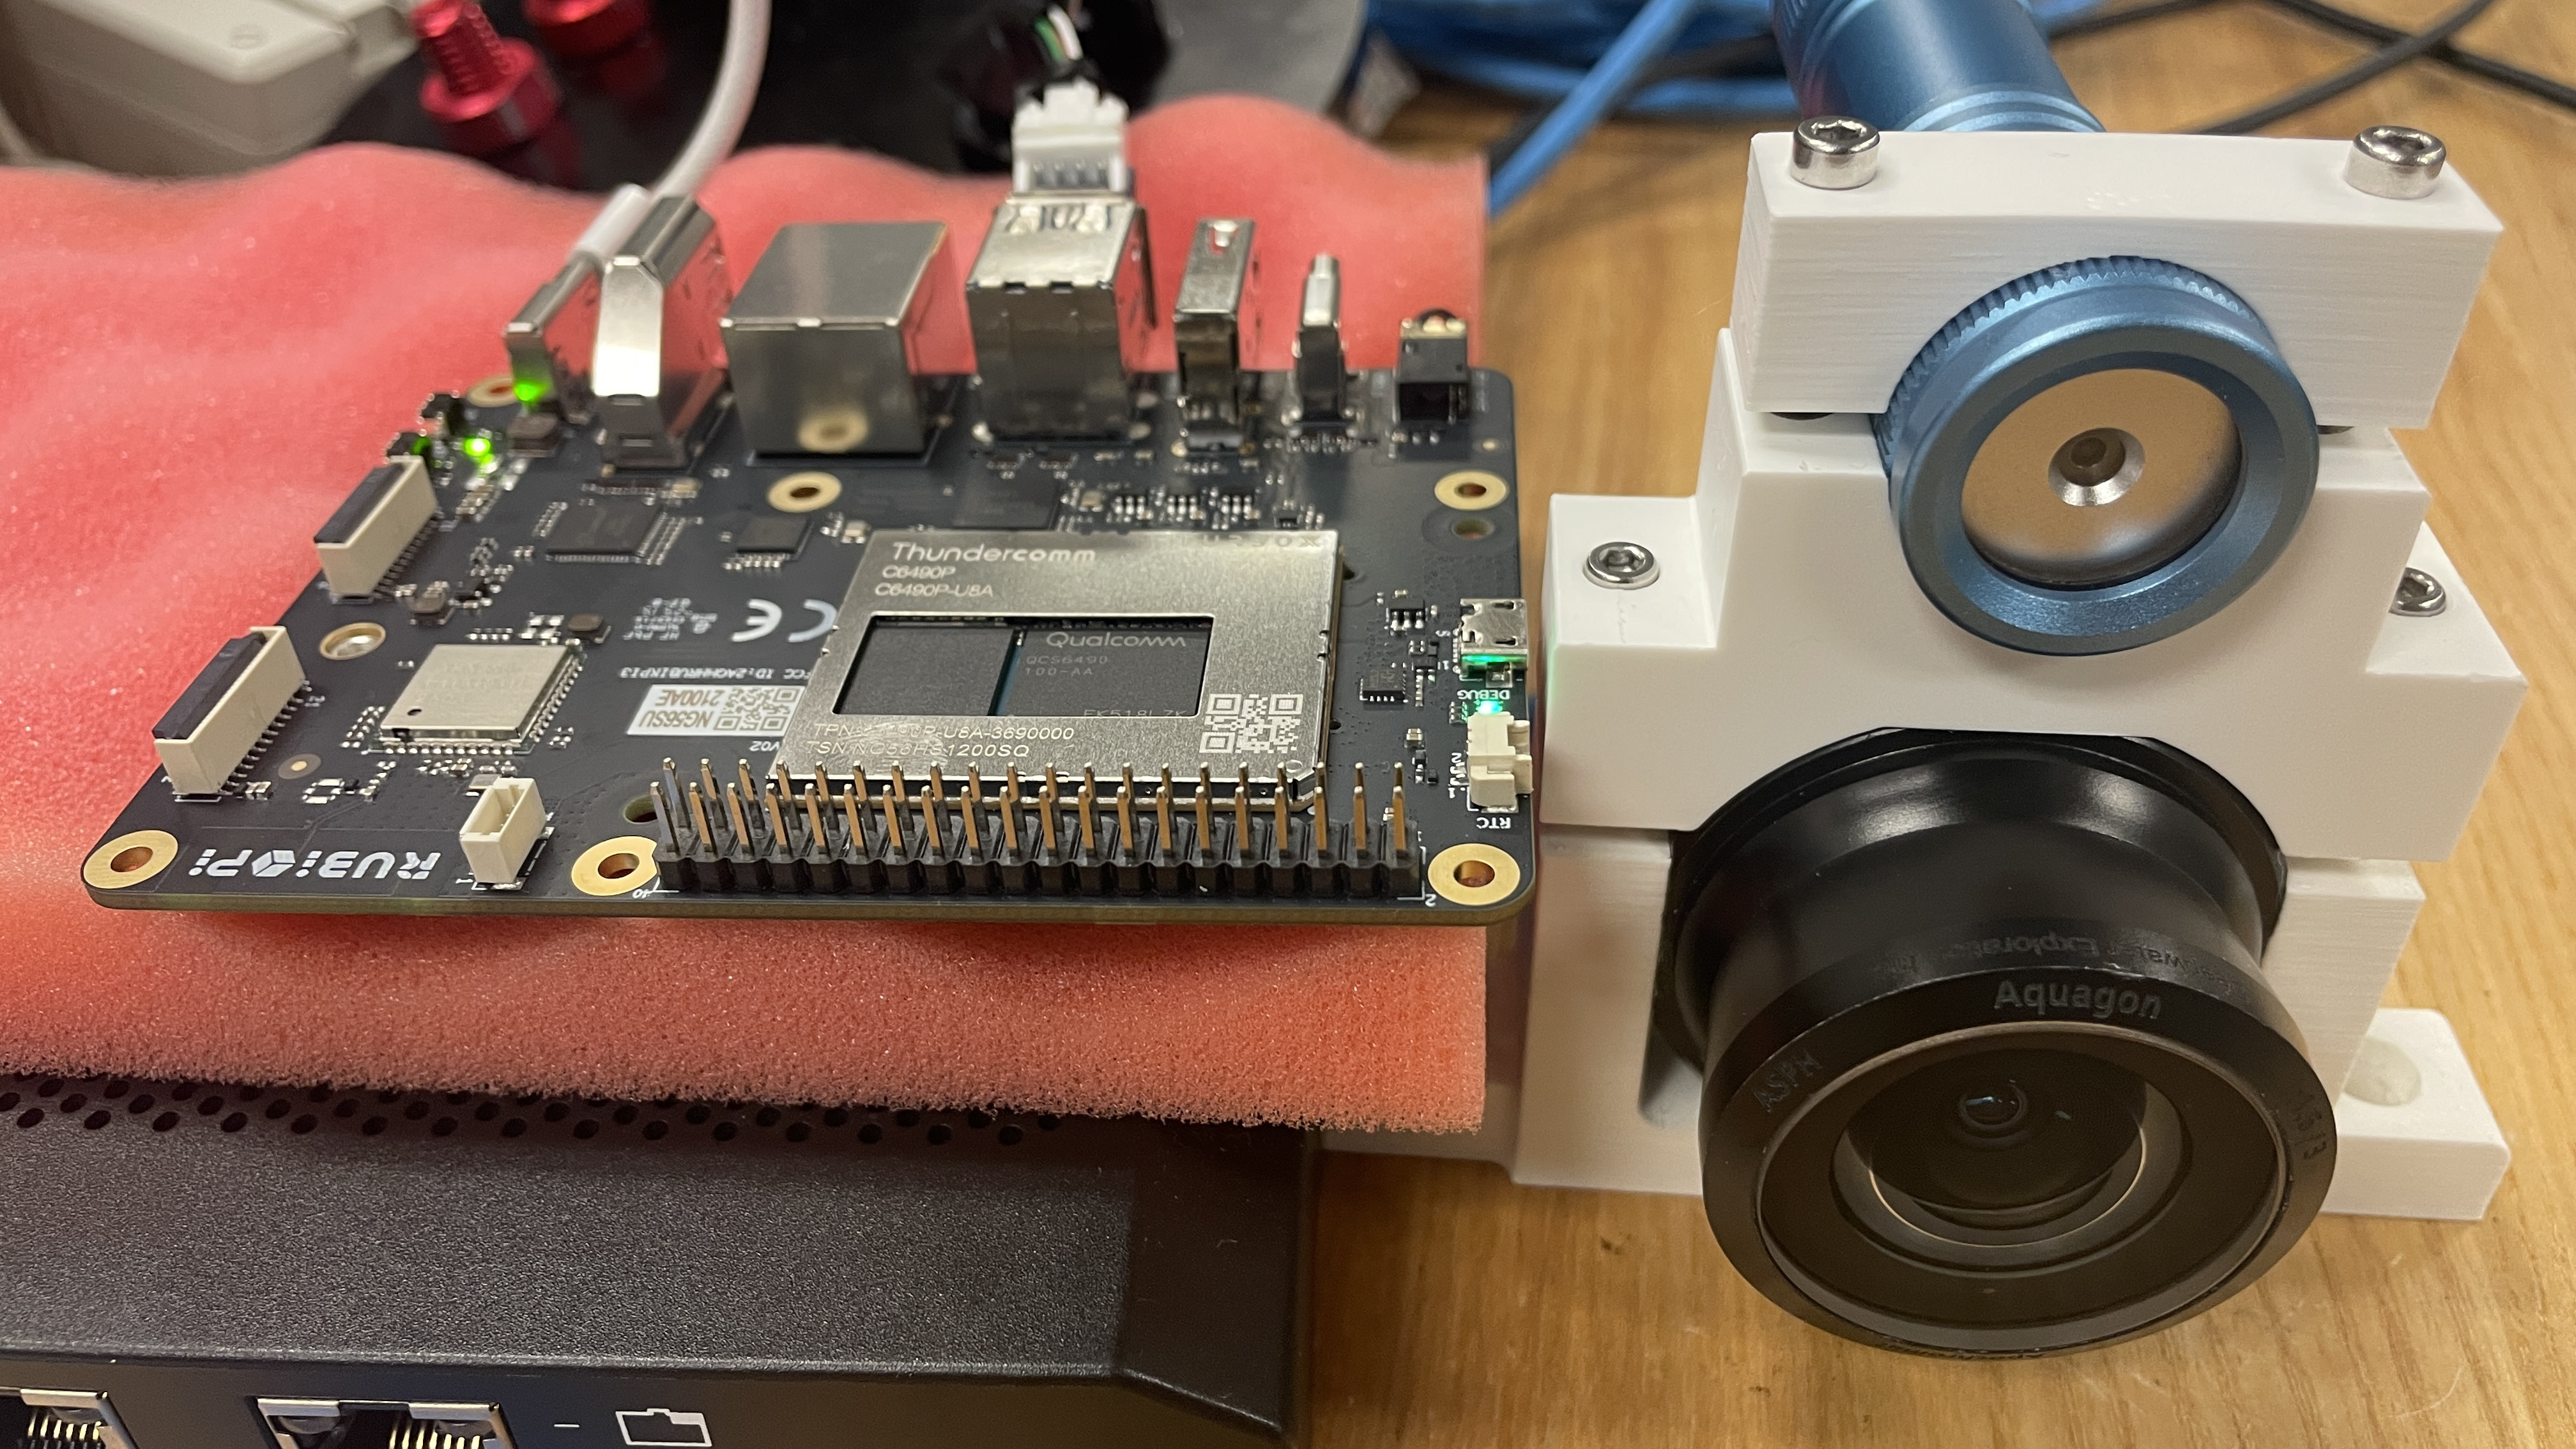
\includegraphics[height=0.7\textheight,width=0.7\textwidth,keepaspectratio]{images/rubik_pi_dwe.png}
\end{frame}

\begin{frame}{GPU Acceleration Setup on Rubik Pi}
   \begin{itemize}
       \item \textbf{Challenge:} Rubik Pi+ Debian 13 lacking Adreno GPU userland drivers
       \item \textbf{Solution:} Bootstrapped Ubuntu Environment
       \item \textbf{Implementation:}
           \begin{itemize}
               \item Configured OpenCL and Vulkan for Adreno GPU support
               \item Built diagnostic tools (\texttt{clinfo}, \texttt{vulkaninfo}) from source
           \end{itemize}
       \item \textbf{Next Step:} Benchmarking GPU performance
   \end{itemize}
   % \centering
   % \includegraphics[height=0.4\textheight,width=0.7\textwidth,keepaspectratio]{}
\end{frame}

\begin{frame}{Rubik Pi Housing}
    \centering
    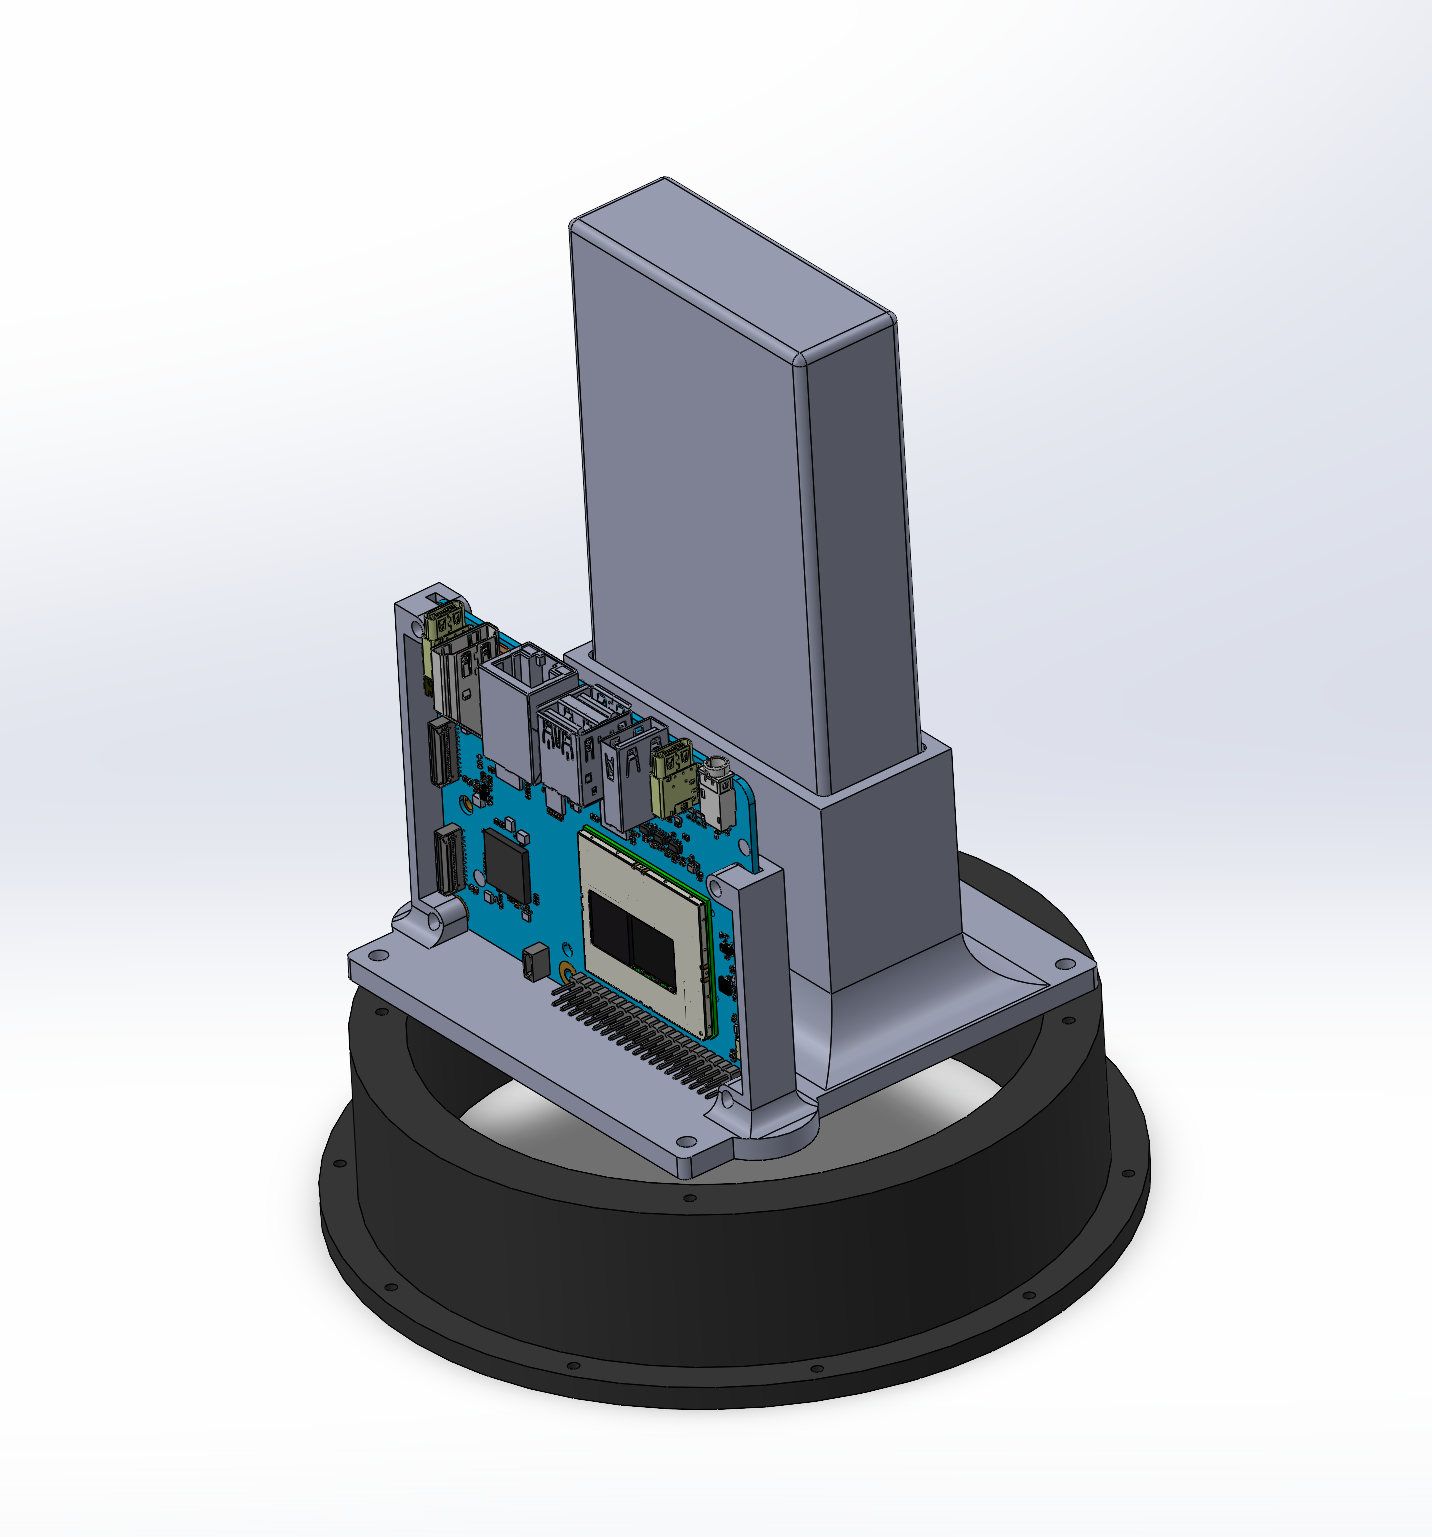
\includegraphics[width=0.4\textwidth,keepaspectratio]{images/rubik_pi_assembly_iso_v1.png}
    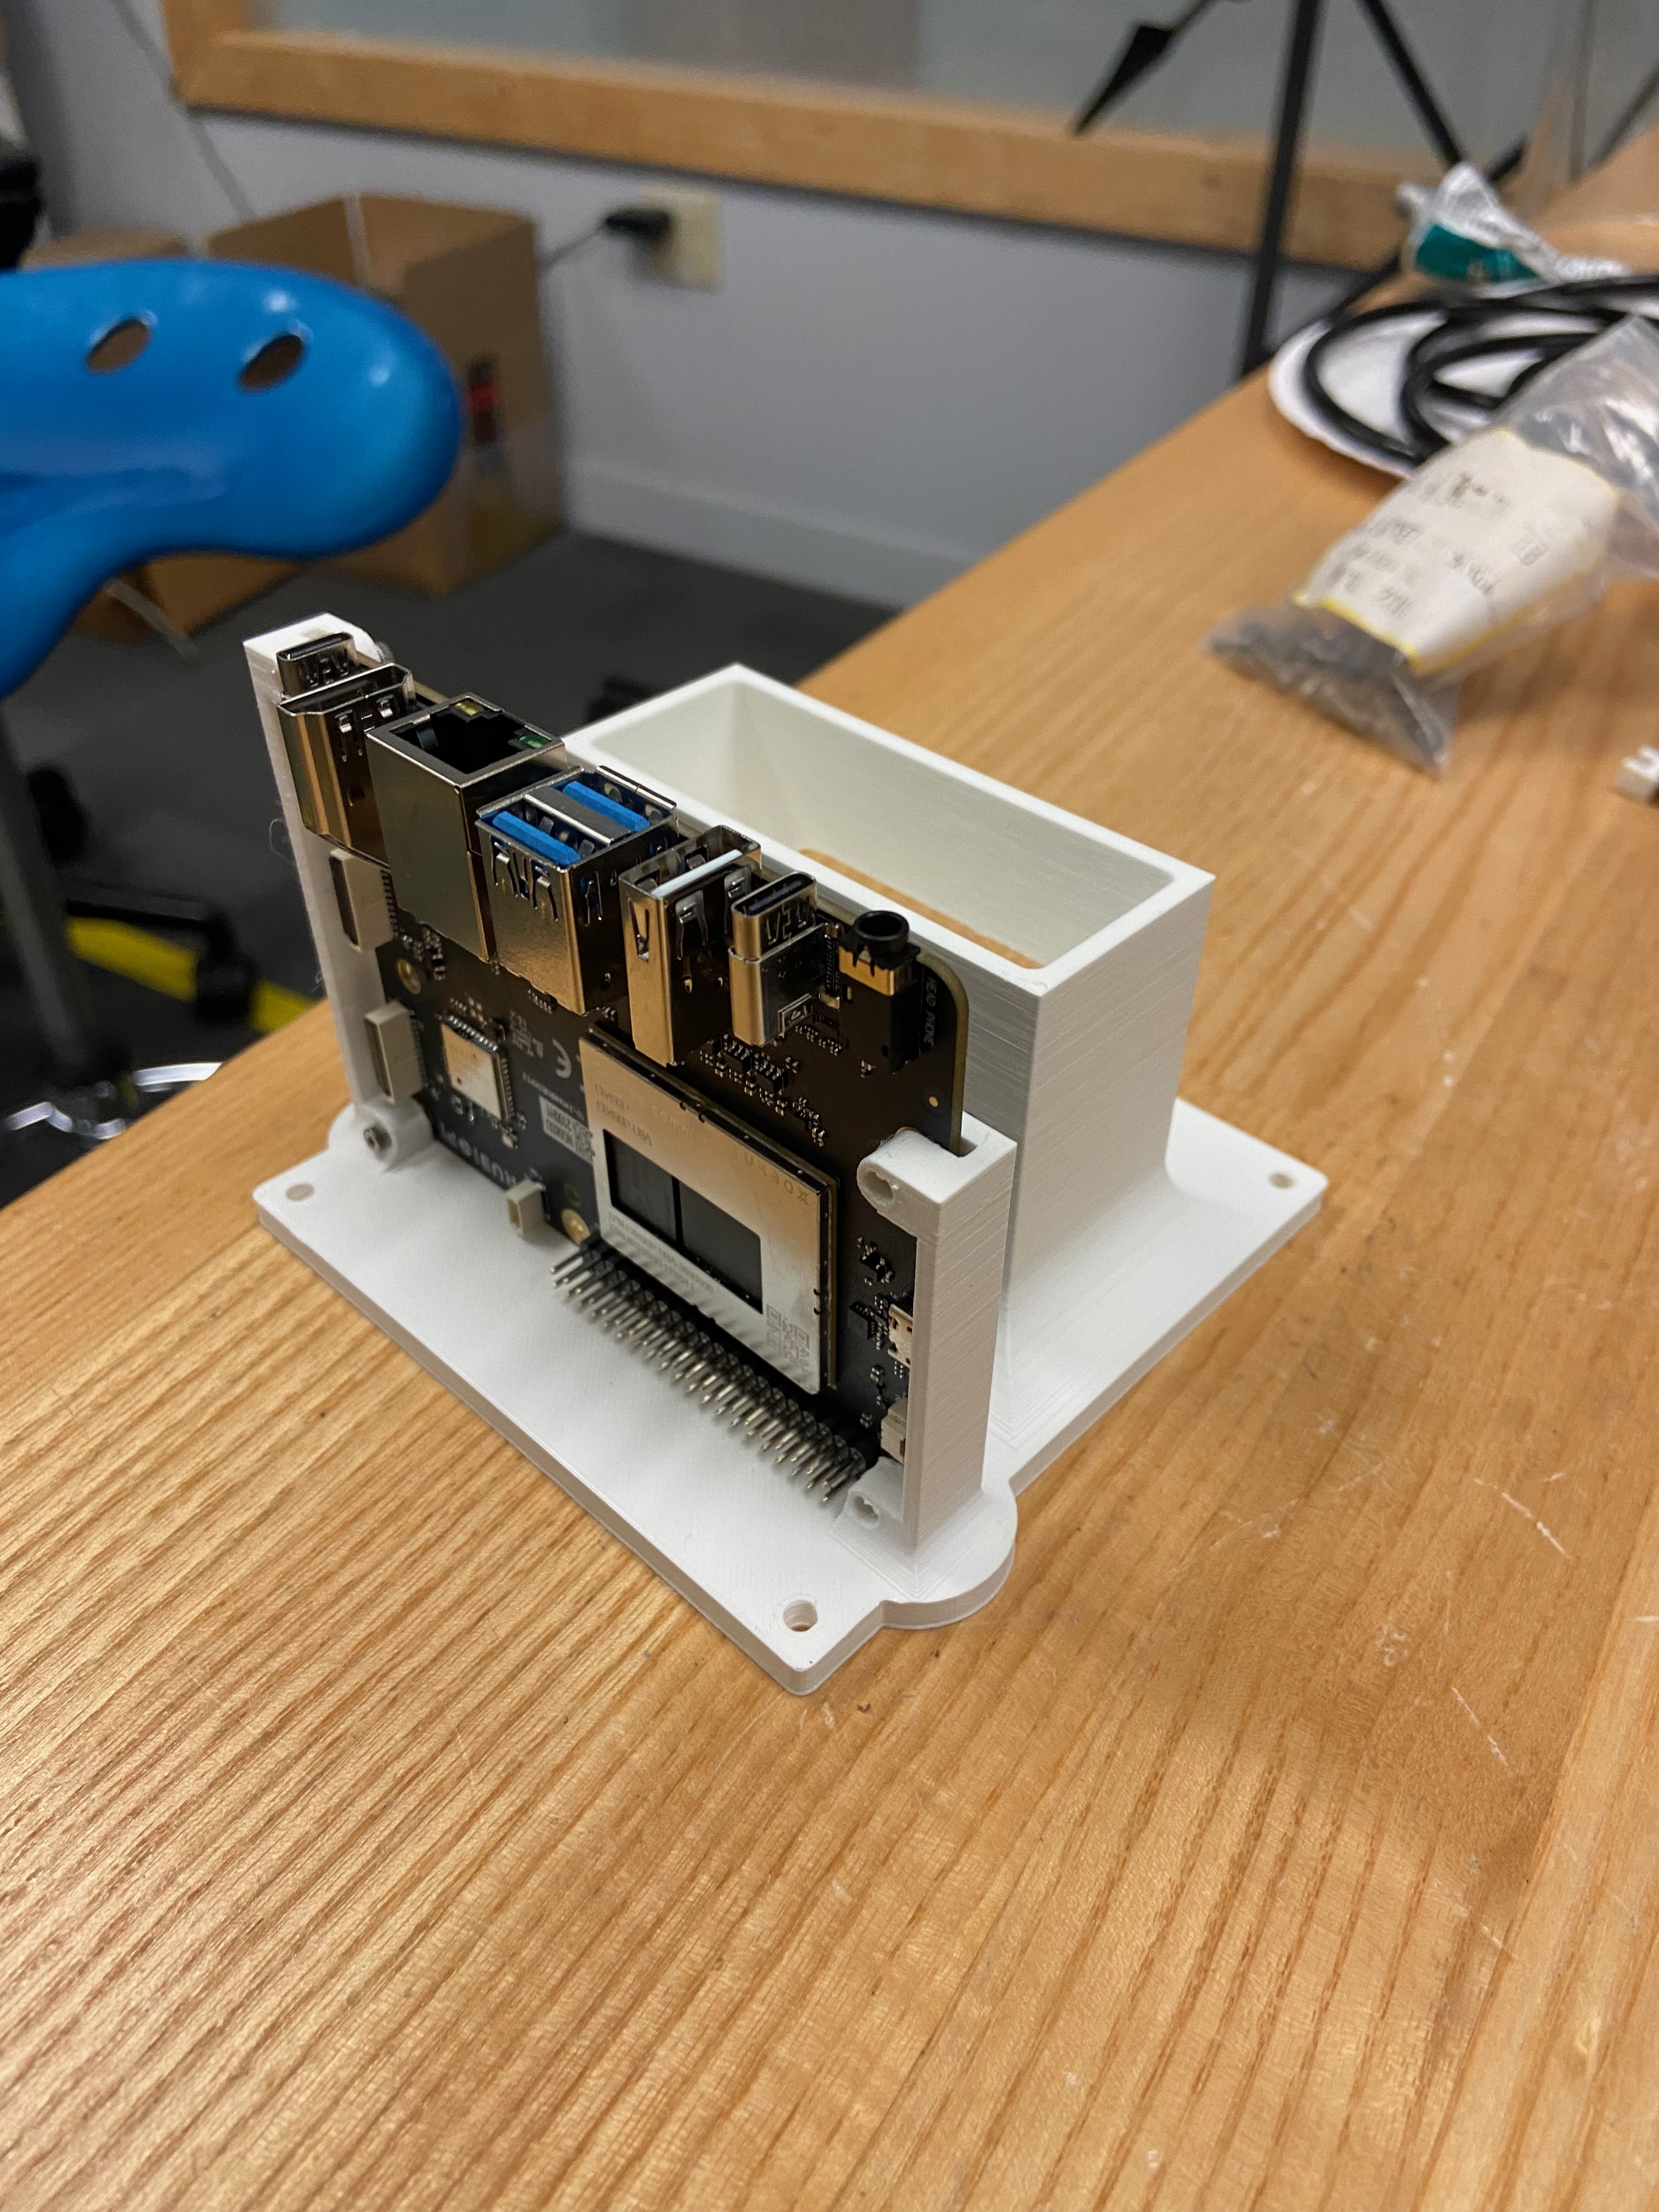
\includegraphics[width=0.4\textwidth, keepaspectratio]{images/rubik_pi_in_housing_v1.jpg}
\end{frame}

\begin{frame}{Enclosure Service}
    \centering
    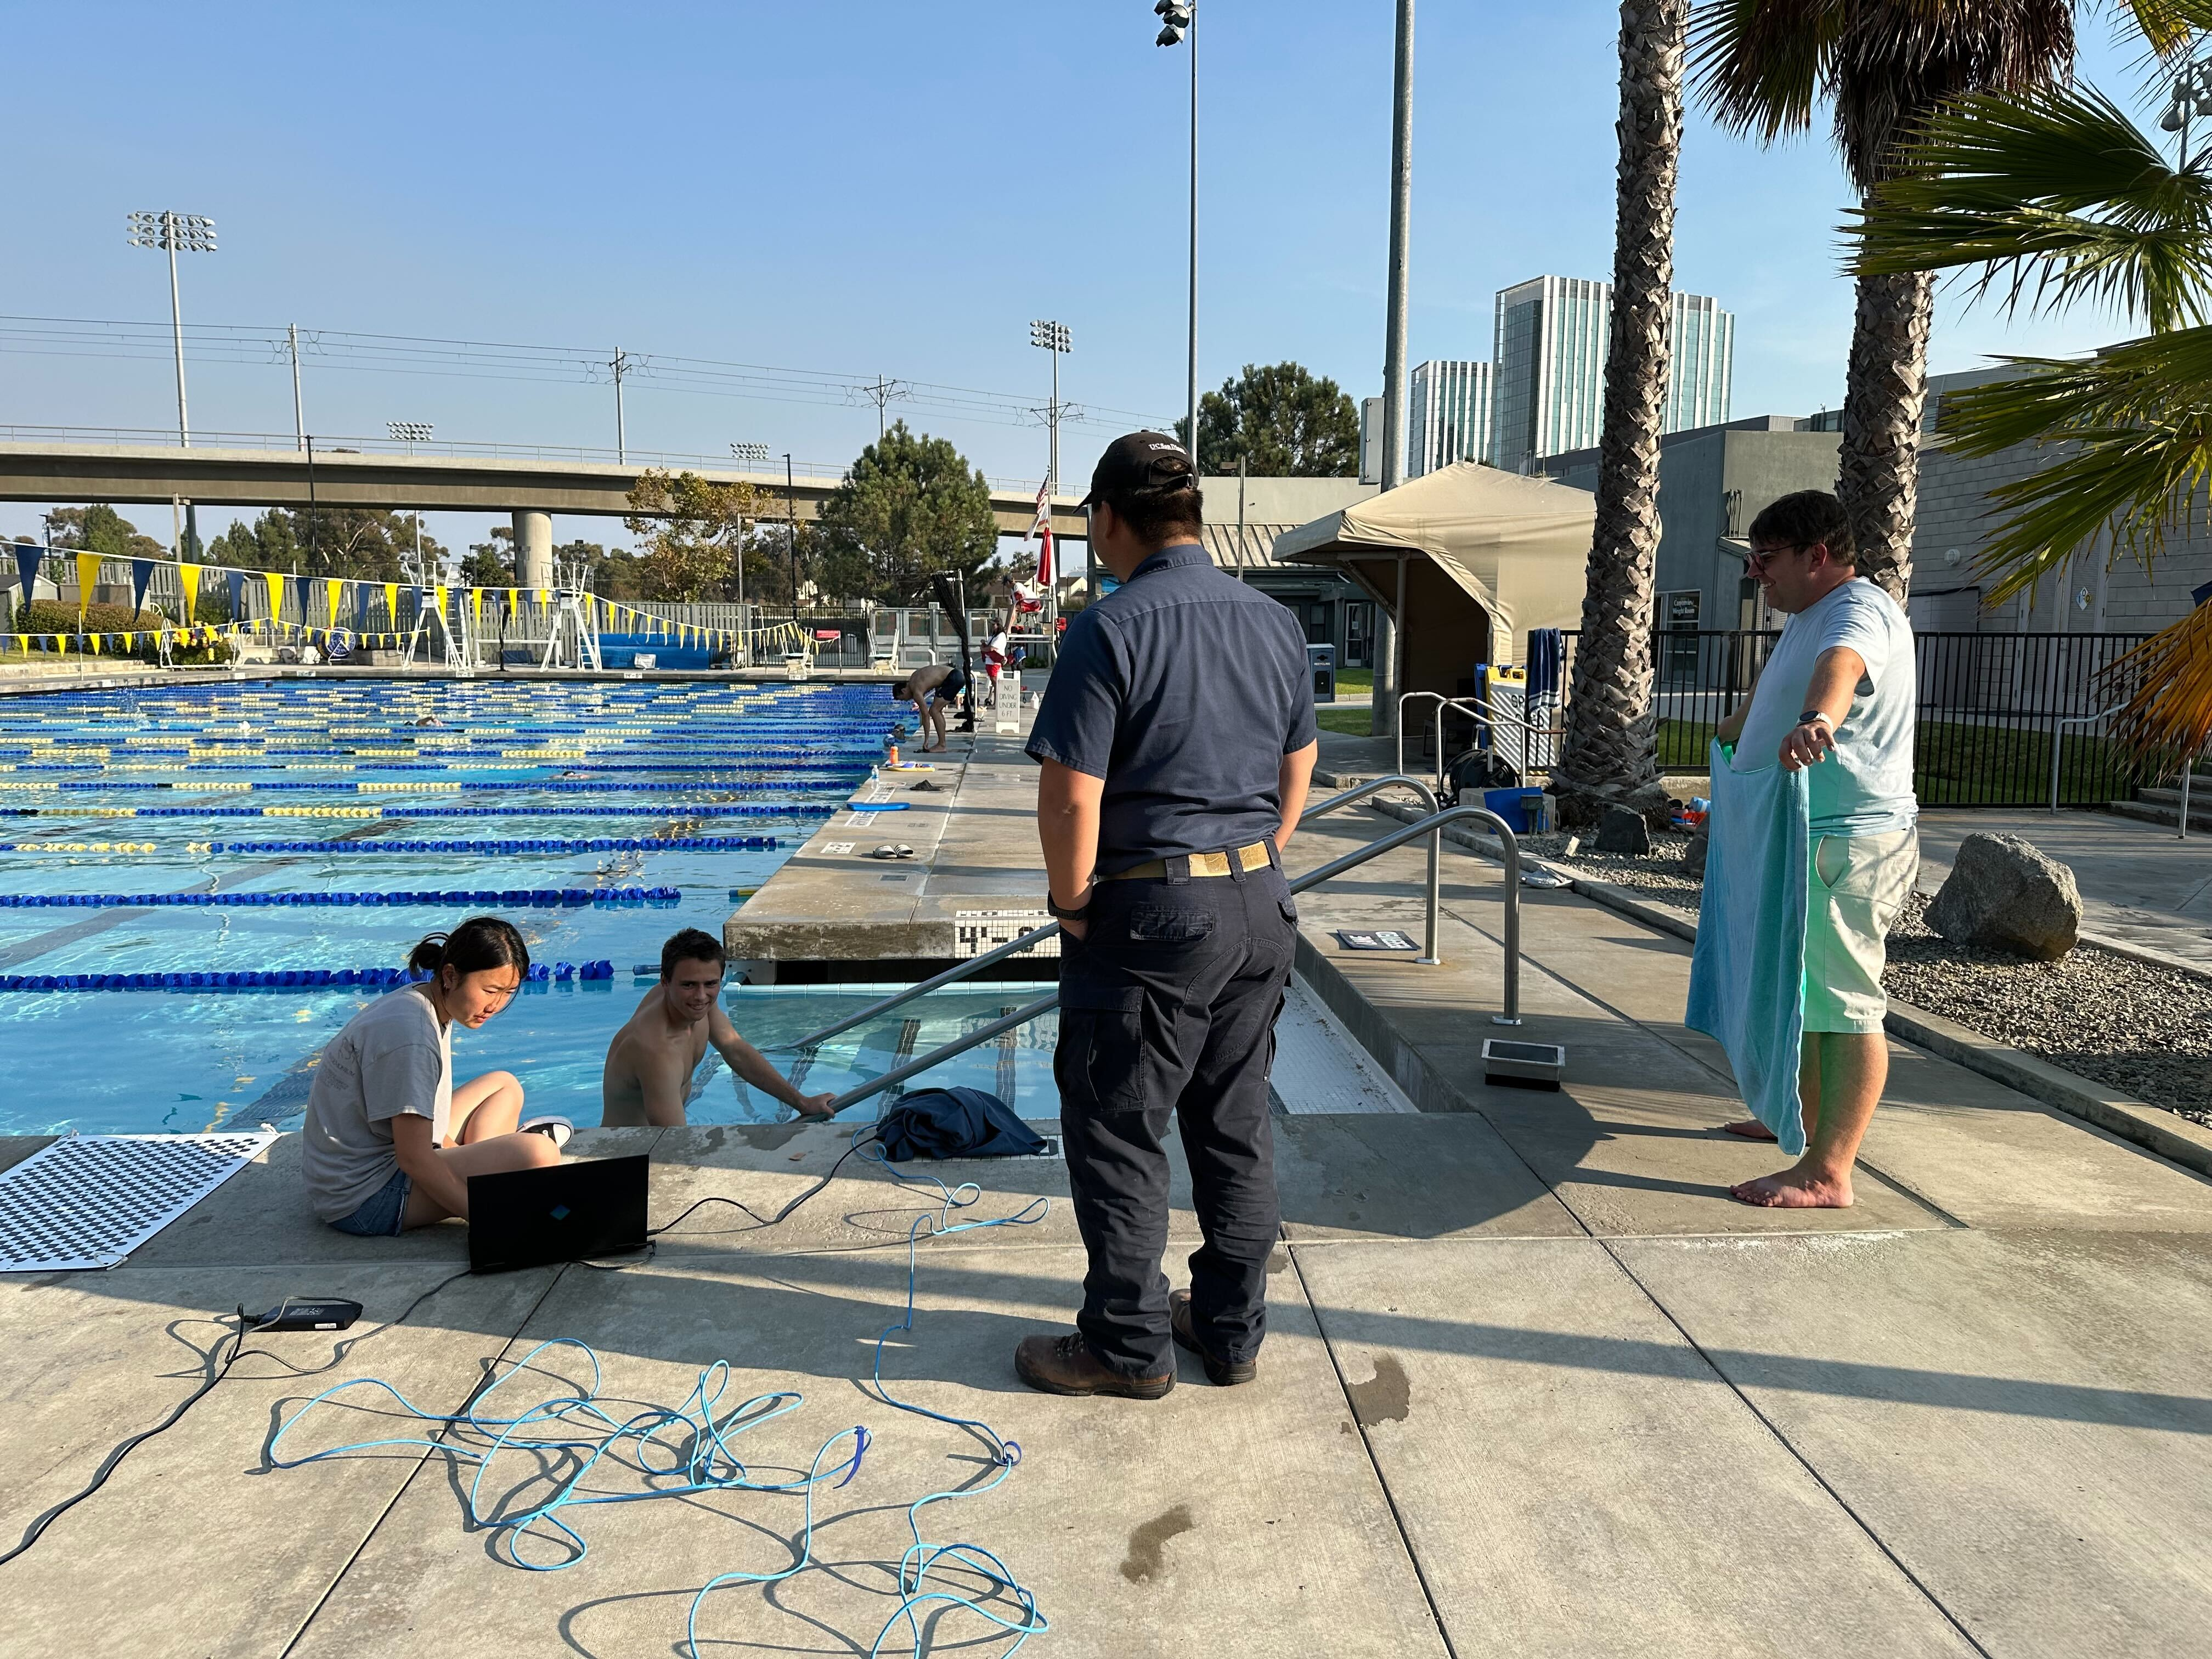
\includegraphics[width=0.4\textwidth,keepaspectratio]{images/towel_pool_testing.jpg}
    \includegraphics[width=0.4\textwidth,keepaspectratio]{images/disassembled_enclosure.png}
\end{frame}

\begin{frame}{SNRGAN For Noise Reduction}
    \vspace{1em} 
    \begin{columns}
        \begin{column}{0.5\textwidth}
            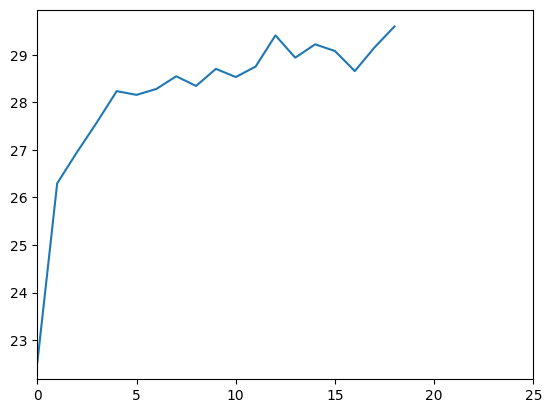
\includegraphics[width=\linewidth,keepaspectratio]{images/psnr-test.png }
        \end{column}
        \begin{column}{0.5\textwidth}
            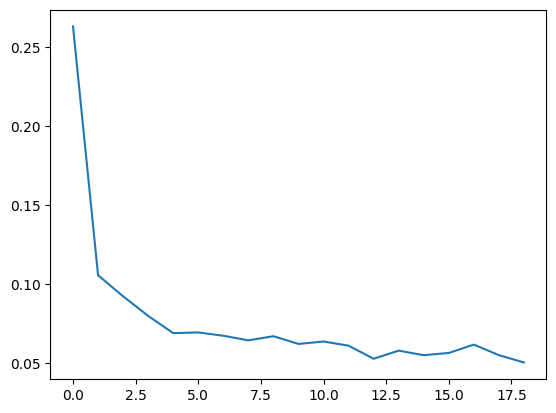
\includegraphics[width=\linewidth,keepaspectratio]{images/nmse-score.png}
        \end{column}
    \end{columns}

    \vspace{0.1em} 
    \begin{center}
        $\mathrm{PSNR} > 30.0\,\mathrm{dB} \ \text{(and upward trend)} \quad \text{and} \quad \mathrm{NMSE} < 0.05$
    \end{center}
\end{frame}

\begin{frame}{SNRGAN Image Outputs}
    \vspace{0.3em} 
    \begin{columns}
        \begin{column}{0.33\textwidth}
            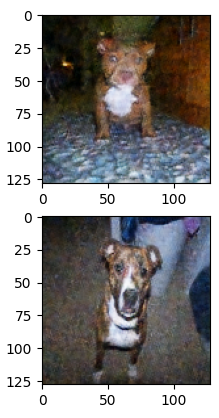
\includegraphics[width=\linewidth,height=0.6\textheight,keepaspectratio]{images/img3.png}
        \end{column}
        \begin{column}{0.33\textwidth}
            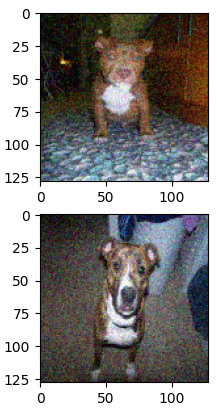
\includegraphics[width=\linewidth,height=0.6\textheight,keepaspectratio]{images/img2.png}
        \end{column}
        \begin{column}{0.33\textwidth}
            
\includegraphics[width=\linewidth,height=0.6\textheight,keepaspectratio]{images/img1.png}
        \end{column}
    \end{columns}
    
    \vspace{0.1em} 
    \begin{itemize}
        \item Used publicly available image datasets (e.g., \textit{Oxford-IIIT Pets}, \textit{Flowers102})
        \item \textbf{MuLA-GAN:} PSNR $\approx 25.59$ dB \textbf{SNRGAN:} PSNR $> 30$ dB
        \item Next step: Use \textit{Underwater Image Enhancement Benchmark Dataset} and aim for lower NMSE and higher PSNR
    \end{itemize}
\end{frame}

\begin{frame}{Fishy Data}
    \begin{columns}
        \begin{column}{0.5\textwidth}
            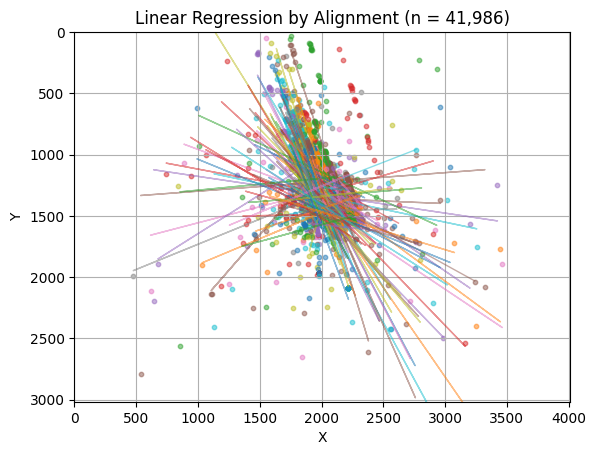
\includegraphics[width=\linewidth,keepaspectratio]{images/regression.png}
        \end{column}
        \begin{column}{0.5\textwidth}
            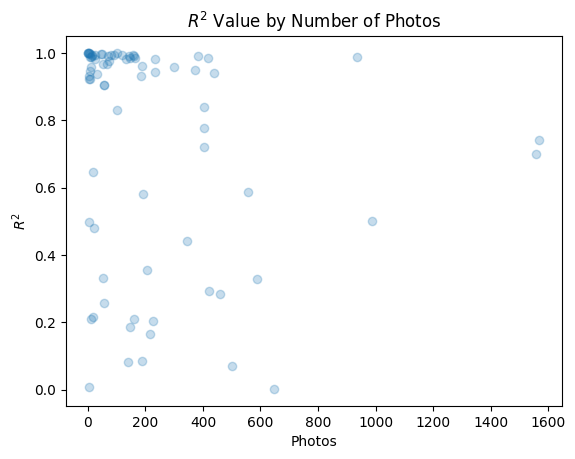
\includegraphics[width=\linewidth,keepaspectratio]{images/rsquare.png}
        \end{column}
    \end{columns}

    \vspace{0.2em} % adjust space above the text
    \begin{center}
        {\small Cutoff $R^2\geq 0.9$ and number of photos $\geq 10$ yields 5592}
    \end{center}
\end{frame}

\begin{frame}{Sensing Fish}
    \begin{columns}
        \begin{column}{0.33\textwidth}
            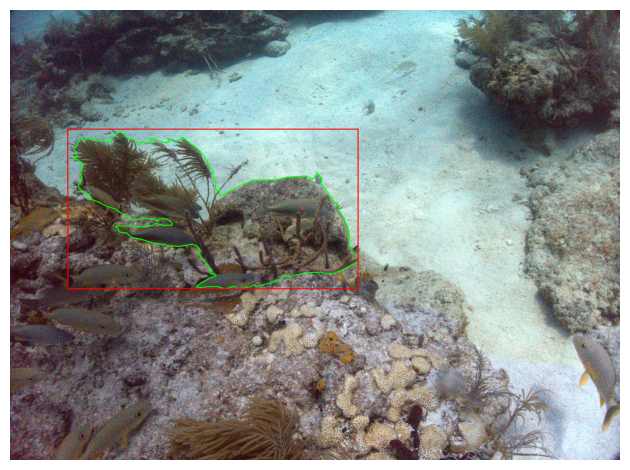
\includegraphics[width=\linewidth,keepaspectratio]{images/original.png}
            {\small Default}
        \end{column}
        \begin{column}{0.33\textwidth}
            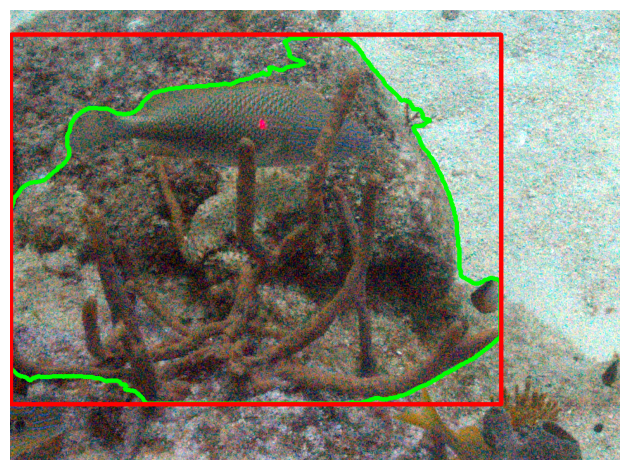
\includegraphics[width=\linewidth,keepaspectratio]{images/current.png}
            {\small Current}
        \end{column}
        \begin{column}{0.33\textwidth}
            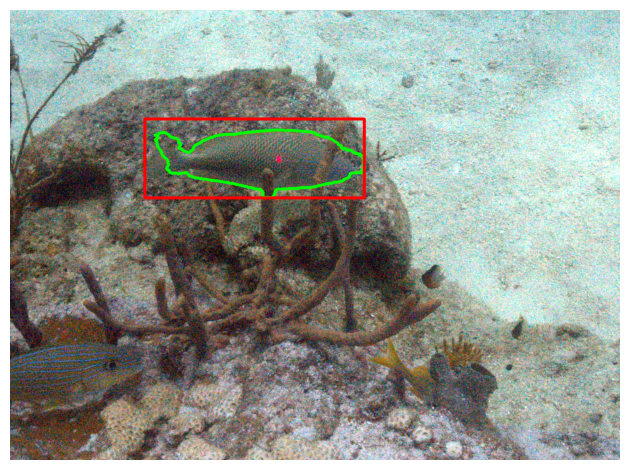
\includegraphics[width=\linewidth,keepaspectratio]{images/ideal.png}
            {\small Goal}
        \end{column}
    \end{columns}
\end{frame}

\begin{frame}{Flat Port Correction}
    \centering
    \item\textbf{Lesson:} Old code is a pain
    
\includegraphics[width=0.6\textwidth,keepaspectratio]{images/remapped.jpg}
\end{frame}


\begin{frame}{FishSense Mobile}
    \begin{columns}[T] % Align columns at the top
        \begin{column}{0.45\textwidth}
            \textbf{Current:}
            \begin{itemize}
                \item Flutter Integration
            \end{itemize}
            \vspace{0.5em}
            \centering
            \includegraphics[width=0.5\linewidth,keepaspectratio]{images/fsmobile.PNG}
        \end{column}
        \begin{column}{0.5\textwidth}
            \textbf{Next Steps:}
            \begin{itemize}
                \item Android integration with Depth Sensing
            \end{itemize}
        \end{column}
    \end{columns}
\end{frame}

